% Template para la realización de la Presentacion de la Tesis.

% Tipo de Documento.
\documentclass[a4paper]{article}

% Idioma.
\usepackage[utf8x]{inputenc}
\usepackage[spanish]{babel}
\usepackage{babelbib}

% Margenes.
\usepackage[outer=4cm,inner=2cm,top=2cm,bottom=2cm]{geometry}
\usepackage{fancyhdr}
\usepackage{lastpage}

% Graficos.
\usepackage{graphicx}
\graphicspath{{./images/}}

% Codigo Fuente.
\usepackage{tabularx}

% Hypervinculos.
\usepackage{url}
\usepackage{color,hyperref}
\definecolor{black}{rgb}{0.0,0.0,0.0}
\definecolor{darkblue}{rgb}{0.0,0.0,0.3}
\hypersetup{colorlinks,breaklinks,
            linkcolor=black,urlcolor=darkblue,
            anchorcolor=darkblue,citecolor=darkblue}

% Guiones
\hyphenation{pro-ble-ma}
\hyphenation{ge-ne-ra-ra}
\hyphenation{pos-te-rior-men-te}

% Paquetes matematicos
\usepackage{amsfonts}
\usepackage{amsmath}
\usepackage{amssymb}
\usepackage{amsthm}
\usepackage{mathrsfs}
\DeclareMathOperator\arctanh{arctanh}

% Definicion de la hoja de firmas.
\newcommand{\signature}[7]{
   \vfill

   \begin{flushright}
      #1, \today
   \end{flushright}
   \vspace{3cm}

   \noindent
   \centering
   \begin{tabularx}{0.9\textwidth}{cXc}
      \multicolumn{3}{c}{\rule{5cm}{1pt}}\\
      \multicolumn{3}{c}{#2}\\
      \multicolumn{3}{c}{#3}\\
      \vspace{3cm}\\
      \rule{5cm}{1pt} & \hspace{2.5cm} & \rule{5cm}{1pt} \\
      #4 & ~ & #5 \\
      #6 & ~ & #7
   \end{tabularx}
   \vspace{1cm}
}

% Encabezado y Titulo del Documento y de la Tesis.
\title{
   {\normalsize
      Universidad de Buenos Aires\\
      Facultad de Ingeniería -- Departamento de Electrónica\\
      Propuesta de Tesis de Ingeniería Electrónica\\
      \vspace{0.7cm}
   }
   Implementación de una Unidad de Punto Flotante basado en el algoritmo BKM
}

% Datos de autor: Tesista, Director y Co-director.
\author{ \textbf{Tesista}                                                           \\
         Ignacio Lesser, \textit{Padrón Nro. 90.942}                                \\
         \texttt{ \href{mailto:ignacio.lesser@gmail.com}{ignacio.lesser@gmail.com}}  \\[2.5ex]
         \textbf{Director}                                                          \\
         Ing. Nicolas Alvarez, \textit{Profesor Adjunto}                            \\
         \texttt{ \href{mailto:nalvarez2001@yahoo.com.ar}{nalvarez2001@yahoo.com.ar}} \\[2.5ex]
         \textbf{Co-director}                                                       \\
         Ing. Octavio Alpago, \textit{JTP. Interino}                                \\
         \texttt{ \href{mailto:oalpago@gmail.com}{oalpago@gmail.com}}               \\[2.5ex]
       }

% Fecha.
\date{\today}

% Pie de Pagina.
\pagestyle{fancy}
\lhead{}
\chead{}
\rhead{}
\lfoot{}
\cfoot{
   {\footnotesize
   \emph{Diseño e implementación de una Unidad de Punto Flotante basada en el algoritmo BKM}\\
   Plan de Tesis -- Página \thepage\ de \pageref{LastPage}
   }
}
\rfoot{}
\renewcommand{\headrulewidth}{0pt}
\renewcommand{\footrulewidth}{0.4pt}

% Documento.
\begin{document}

\maketitle

%\thispagestyle{empty}

%\begin{abstract}
%\end{abstract}

\thispagestyle{fancy}

\section{Objeto y Área de la Tesis}

El objetivo principal de este trabajo consiste en diseñar e implementar en hardware digital una unidad de punto flotante basada en el algoritmo BKM. Dicho diseño e implementación será realizado a través del uso del lenguaje de descripción de hardware Verilog, y su síntesis en un dispositivo FPGA \footnote{\label{FPGA}Field Programmable Gate Array: dispositivo semiconductor que contiene bloques de lógica cuya interconexión y funcionalidad puede ser configurada `in situ' mediante un lenguaje de descripción especializado.}.
El interés en este desarrollo proviene de la necesidad de crear un unidad de punto flotante eficiente y con gran capacidad de calculo para utilizarse como periférico de un microprocesador diseñado en la misma facultad. Con este proyecto no solamente se logra cubrir las operaciones básicas de una FPU sino que se va un paso mas lejos y se agregan un serie de operaciones extras que expanden las funcionalidad de la unidad así como también la posibilidad de trabajar en el campo de los números
complejos . Estas características surgen naturalmente al utilizar el algoritmo BKM.
La principal ventaja de utilizar una FPU es la capacidad de implementar operaciones matemáticas complejas en tiempo real.

El área profesional de relevancia de la presente tesis es el diseño de sistemas digitales y su aplicación en el ámbito de las microprocesadores, aunque no se limita sólo a ese ámbito. Una vez comprendido el funcionamiento del algoritmo y analizado sus características se podrá utilizar el conocimiento en la aplicación práctica en hardware de algoritmos de procesamiento de señales en general.

\newpage

\section{Introducción. Antecedentes}

\subsection{Unidad de punto flotante}
Hablar sobre  FPU???? hace falta explicar xq se necesita una? o sobre su historia?
%Empezar hablando sobre una FPU y xq conviene tener una y sus ventajas. Pasar la linea sobre la capacidad de implementar operaciones matematicas complejas en tiempo real aca??


%El costo, tamaño y potencia de los circuitos electrónicos fue relativamente alto a lo largo de 
%Mathematician John von Neumann proposed the ALU concept in 1945 in a report on the foundations for a new computer called the EDVAC.[1]
%The cost, size, and power consumption of electronic circuitry was relatively high throughout the infancy of the information age. Consequently, all serial computers and many early computers, such as the PDP-8, had a simple ALU that operated on one data bit at a time, although they often presented a wider word size to programmers. One of the earliest computers to have multiple discrete single-bit ALU circuits was the 1948 Whirlwind I, which employed sixteen of such "math units" to enable it to operate on 16-bit words.
%In 1967, Fairchild introduced the first ALU implemented as an integrated circuit, the Fairchild 3800, consisting of an eight-bit ALU with accumulator.[2] Other integrated-circuit ALUs soon emerged, including four-bit ALUs such as the Am2901 and 74181. These devices were typically "bit slice" capable, meaning they had "carry look ahead" signals that facilitated the use of multiple interconnected ALU chips to create an ALU with a wider word size. These devices quickly became popular and were widely used in bit-slice minicomputers.
%Microprocessors began to appear in the early 1970s. Even though transistors had become smaller, there was often insufficient die space for a full-word-width ALU and, as a result, some early microprocessors employed a narrow ALU that required multiple cycles per machine language instruction. Examples of this include the original Motorola 68000, which performed a 32-bit "add" instruction in two cycles with a 16-bit ALU, and the popular Zilog Z80, which performed eight-bit additions with a four-bit ALU.[3] Over time, transistor geometries shrank further, following Moore's law, and it became feasible to build wider ALUs on microprocessors.
%Modern integrated circuit (IC) transistors are orders of magnitude smaller than those of the early microprocessors, making it possible to fit highly complex ALUs on ICs. Today, many modern ALUs have wide word widths, and architectural enhancements such as barrel shifters and binary multipliers that allow them to perform, in a single clock cycle, operations that would have required multiple operations on earlier ALUs.

%In the 1980s, it was common in IBM PC/compatible microcomputers for the FPU to be entirely separate from the CPU, and typically sold as an optional add-on. It would only be purchased if needed to speed up or enable math-intensive programs.
%There are also add-on FPUs coprocessor units for microcontroller units (MCUs/µCs)/single-board computer (SBCs), which serve to provide floating-point arithmetic capability. These add-on FPUs are host-processor-independent, possess their own programming requirements (operations, instruction sets, etc.) and are often provided with their own integrated development environments (IDE)s.

\subsection{Algoritmo BKM}

El algorito BKM \cite{BKM} fue desarrollado en 1994 por Jean-Claude Bajard, Sylvanus Kla y Jean-Michel Muller (con las primeras letras de cada apellido se puede formar la sigla BKM) y es parte de la familia de los denomidados algoritmos de desplazamiento y suma o \textit{Shift and add algorithms} en inglés. Estos algoritmos intentan explotar características particulares de un problema para poder reducirlo en operaciones simples como sumas y desplazamientos. Estas operaciones pueden ser implementadas muy facilmente en un circuito digital lo que permite reducir considerablemente la complejidad del circuito a utilizar.

El algoritmo BKM está intimamente relacionado con el método de Brigss para el cálculo del logaritmo (Henry Brigss, 1600 apróx.) y el algoritmo CORDIC \cite{Volder} creado por Jack E. Volder en 1956. De manera simplista se lo puede pensar como una mejora del último, ya que resuelve un problema muy similar pero con numerosas mejoras y/o ventajas (ACA TENGO QUE PONER ALGO SOBRE LAS VENTAJAS?? O LO DEJO PARA LA TESIS?).

El algoritmo de Briggs para el cálculo de $\ln(x)$ dice que si se encuentra una secuencia $d_k$ tal que la productoria de $x$ con $(1+d_k 2^{-k})$ es cercana a 1 entonces vale que:

\begin{equation} \label{eq:briggs_ln}
   \begin{subequations}
      \begin{aligned}
         x \prod_{k=1}^{n} (1+d_k 2^{-k}) \approx 1     \\
         \ln(x) \approx - \sum_{k=1}^{n} \ln(1+d_k 2^{-k})
      \end{aligned}
   \end{subequations}
\end{equation}

El algoritmo CORDIC realizaba rotaciones en coordenadas circulares. Partiendo de esa base es fácil extender su funcionamiento para que realice rotaciones en coordenadas hiperbólicas y lineales \cite{Walther}. Para lograrlo se agrega una variables que modifica las ecuaciones y además se eligen diferentes angulos para el acumulador de angule (variable z del algoritmo).
Las ecuaciones del CORDIC completo son:

\begin{equation} \label{eq:cordic_eq}
   \begin{subequations}
      \begin{aligned}
         x_{n+1} &=  x_n - m \cdot d_n \cdot 2^{-n}   \\
         y_{n+1} &=  y_n + d_n \cdot 2^{-n}             \\
         z_{n+1} &=  z_n - d_n \cdot \alpha_{m,n}
      \end{aligned}
   \end{subequations}
\end{equation}

Donde $N$ representa la cantidad de pasos del algoritmo y se cumple que $n= 0, 1, 2, ... , N-1$. $\alpha_{m,n}$ representa los angulos rotados para las diferentes coordenadas. $d_n$ es una variable de control que maneja los sumadores/restadores.

   Consideremos el paso básico del algoritmo CORDIC en modo trigonométrico (con m=1).
   Si definimos el número complejo $E_n = x_n + j \, y_n$ con $j=\sqrt{-1}$, obtenemos $E_{n+1} = E_n (1+j \, d_n 2^{-n})$, esta relación es similar al paso básico del algorithmo de Briggs.
   Esta similitud nos lleva a una generalización de ese algoritmo: podriamos realizar multiplicaciones por terminos $(1+d_n 2^{-n})$, donde los $d_n$s son números complejos elejidos de tal manera que la multiplicación por $d_n$ pueda reducirce a unas pocas sumas.
   Entonces se define el algoritmo BKM de la siguiente manera:

\begin{equation} \label{eq:bkm_eqs}
   \left\{
      \begin{aligned}
         E_{n+1} &= E_n \cdot (1 + d_n 2^{-n})   \\
         L_{n+1} &= L_n - \ln(1 + d_n 2^{-n})
      \end{aligned}
   \right.
\end{equation}


   con $d_n = d_n^r + j d_n^i $ y $d_n^r, d_n^i \in \{ 0, \pm 1 \}$ y $\ln z = t$ es el número complejo $t$ tal que $\exp{t} = z$ y cuya parte imaginaria está entre $-\pi$ y $\pi$.
   Este algoritmo nos permitirá calcular de manera natural logaritmos y exponenciales en el campo de los números complejos.


\section{Desarrollo previsto de la Tesis}

\subsection{Teoría, enfoque y métodos a utilizar}

El enfoque de la tesis se basará en una parte teórica y una experimental.
Se analizarán los modelos y desarrollos algorítmicos para la implementación del algoritmo BKM y luego se realizará un análisis para el diseño de un IP core que ponga en práctica uno de ellos. Una vez codificado el hardware, se procederá a realizar su síntesis en un dispositivo FPGA utilizando un kit de desarrollo, se realizarán los bancos de prueba correspondientes y se analizarán los resultados obtenidos.

\subsection{Estudios conexos}

Asignaturas y otros estudios previstos que son relevantes al desarrollo de la Tesis.

\begin{itemize}
   \item \textbf{Sistemas Digitales:} Asignatura que abarca la teoría de técnicas de diseño de hardware digital y codificación de sistemas digitales, así como también su síntesis y medición.
   \item \textbf{Procesamiento de Señales:} Asignatura que abarca los conceptos respecto a la implementación de los algoritmos.
\end{itemize}

\subsection{Alcance proyectado para la tesis}

Como resultados a obtener de la presente tesis se tienen los siguientes:

\begin{itemize}
   \item Código fuente completamente sintetizable del diseño y todos sus subbloques.
   \item Ejemplos de instanciación.
   \item Scripts de simulación.
   \item Bancos de prueba, incorporando chequeos automáticos del tipo PASA/FALLA.
   \item Resultado de mediciones pertinentes al diseño del IP.
   \item Hoja de datos.
   \item Detalle de la arquitectura usada.
   \item Análisis comparativo de procesamiento entre el IP desarrollado y desarrollos de terceros.
   \item Proposición de trabajos futuros y/o mejoras.
\end{itemize}

Para asegurar que el proyecto de tesis incluya todos los trabajos requeridos, los procesos a completar se describen en un plan de trabajo en la siguiente sección.

\newpage

\subsection{Plan de trabajo}

%Planificación y definición: descomponer la totalidad de la tesis en las tareas, procesos y fases, necesarios para lograr el resultado. Indicar cómo se definirá, verificará y controlará el alcance previsto de la tesis. Incluir un plan de trabajo tentativo, estimando los plazos de ejecución de cada parte.

La duración total del trabajo se estima en un año y se considera que la misma estará compuesta por las siguientes etapas:

\begin{itemize}
    \item \textbf{Investigación Bibliográfica:} Recolección de Libros, Papers, Trabajos de Tesis, y fuentes de investigación con el objetivo de obtener el entendimiento teórico requerido y conocer el estado del arte en el tema a trabajar.
    \item \textbf{Introducción al trabajo de tesis:} Comprender la teoría de una unidad de una FPU y del algoritmo BKM. Describir el contenido teórico requerido para exponer los conceptos de funcionamiento del hardware a desarrollar.
    \item \textbf{Análisis de Arquitecturas:} Analizar las diferentes arquitecturas digitales propuestas para implementar el sistema. Elegir en base a un criterio una de ellas para realizar el desarrollo.
    \item \textbf{Estudio de mejoras:} Estudiar la factibilidad de realizar una mejora a la arquitectura antes mencionadas.
    \item \textbf{Implementación:} Implementar la arquitectura seleccionada en Verilog y desarrollar los bancos de prueba de simulación para verificar su correcta funcionalidad. Se generará un IP core en RTL para implementar el sistema. Dicho RTL cumplirá con ciertas condiciones de portabilidad y legibilidad del código para que el mismo sea efectivamente un IP core.
    \item \textbf{Verificación y validación:} Experimentar el IP core en un ambiente de simulación y en campo. Realizar la síntesis de la misma para distintos dispositivos FPGA, medir recursos utilizados, máxima frecuencia de operación y potencia consumida.
    \item \textbf{Conclusiones y Trabajos a Futuro:} Se extraerán las conclusiones pertinentes sobre los resultados obtenidos y se propondran futuras mejoras de la arquitecturas (si correspondiese) a partir de los resultados obtenidos.
    \item \textbf{Preparación del Informe Final:} Se consolidará la documentación con la memoria de la tesis la cual contendrá el resultado de todo el trabajo realizado. Se revisará la tesis por el director y por los pares antes de enviarla al jurado.
    \item \textbf{Preparación de la presentación y defensa de la Tesis:} Se preparará la presentación (diapositivas) con los objetivos, alcance, introducción, desarrollo de la arquitectura, resultados obtenidos, conclusiones y trabajos a futuro. La misma será posteriormente utilizada para la defensa.
\end{itemize}

En la figura \ref{TablaActividades} se encuentra el plan propuesto para la formación del tesista y el cumplimiento de los objetivos.

\begin{figure}[h!]
   \label{TablaActividades}
   %trim option's parameter order: left bottom right top
   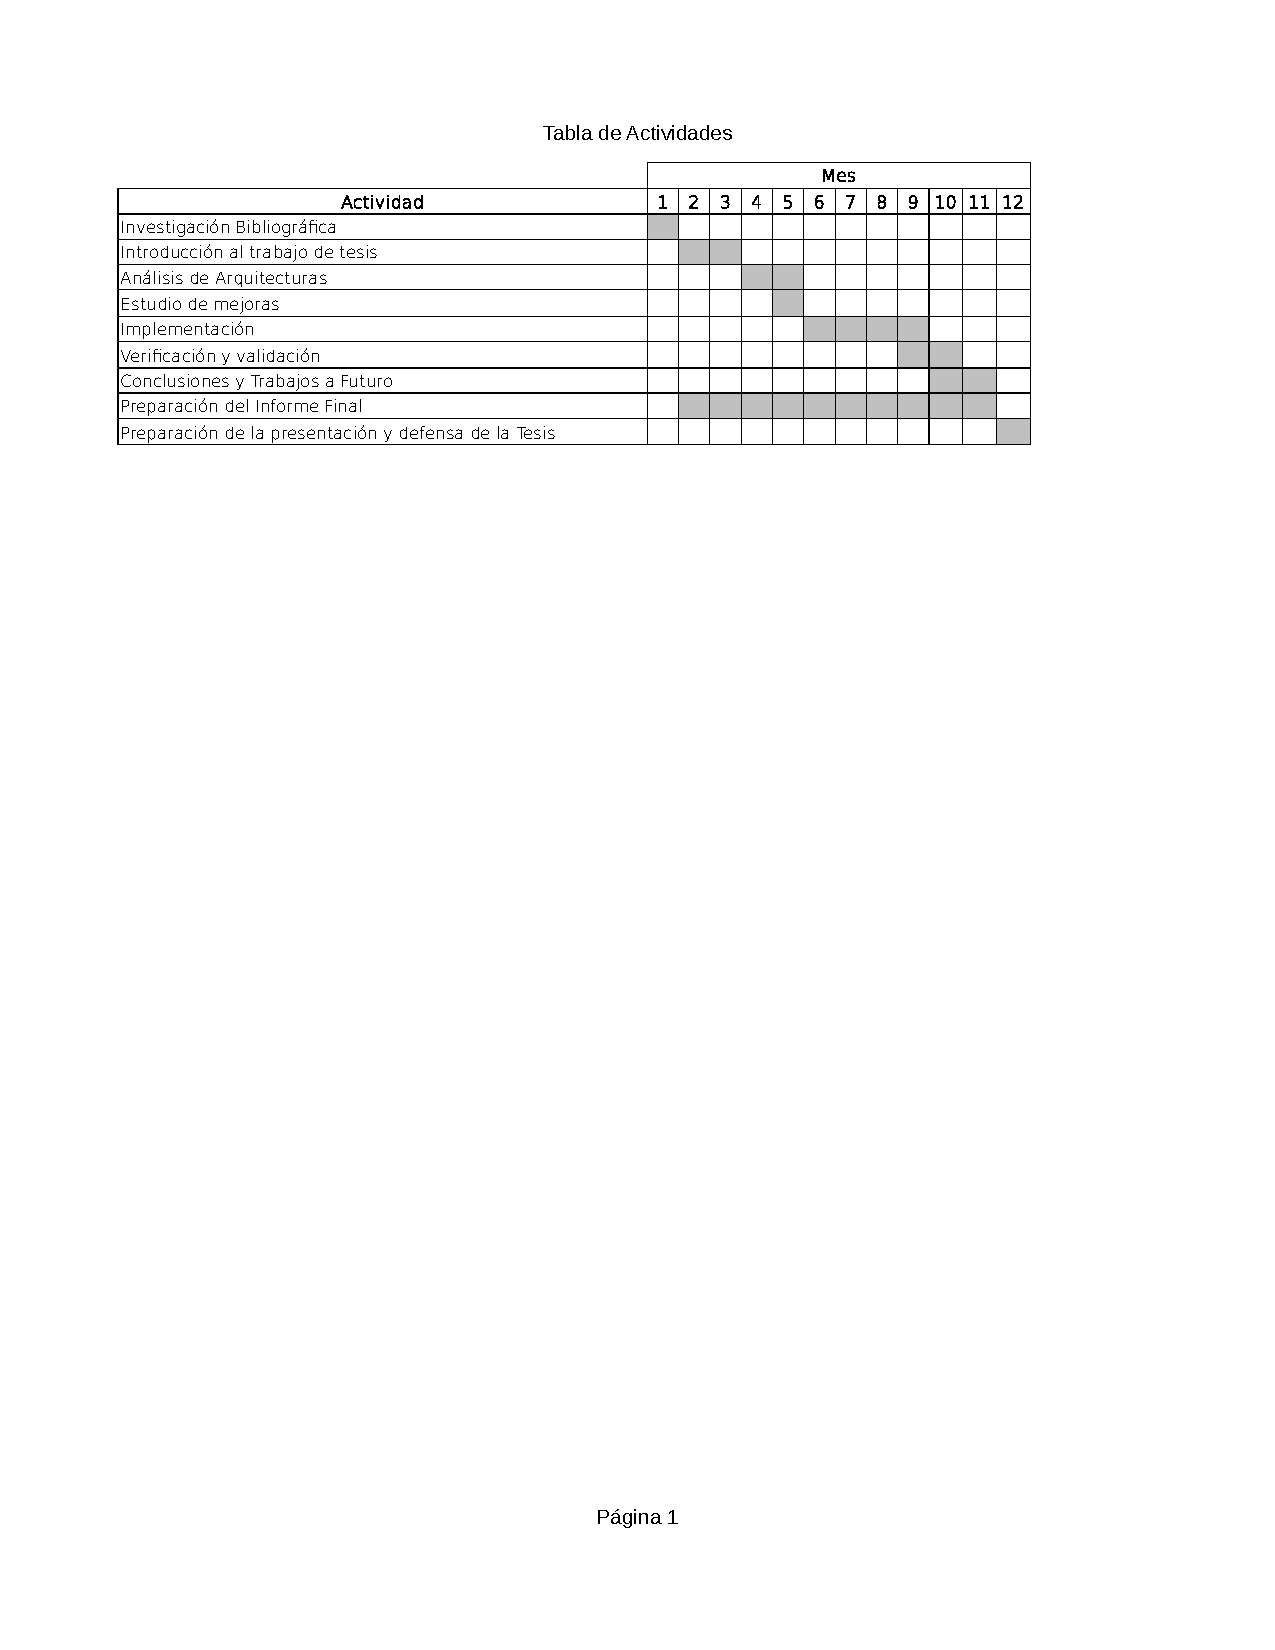
\includegraphics[trim = 20mm 200mm 20mm 25mm, clip, width=\textwidth]{tabla_actividades}
   \caption{Diagrama de las actividades a realizar por el tesista.}
\end{figure}

\newpage

\section{Bibliografía}

\begin{thebibliography}{99}

\bibitem{BKM} J.M. Muller, J.C. Bajard y S. Kla, ``BKM: a new hardware algorithm for complem elementary functions'', IEEE Transactions on Computers, 1994.
\bibitem{Volder} J. Volder, ``The cordic computing technique'', IRE Trans. Elect. Comput., 1959. Reimpreso en Computer Arithmetic, vol. 1, E.E. Swartzlander, Ed. CA: IEEE Computer Society Press Tutorial, 1990.
\bibitem{Walther} J. Walther, ``A unified algortithm for elemetary functions'', Joint Comput. Conf. Proc., 1971. Reimpreso en Computer Arithmetic, vol. 1, E.E. Swartzlander, Ed. CA: IEEE Computer Society Press Tutorial, 1990.
% agregar aca el 
%\bibitem{Wakerly} John F. Wakerly, ``Diseño Digital - Principios y Prácticas'', Tercera Edición, Pearson, 2010.
%\bibitem{Hennesy - Patterson} John L. Hennessy \& David A. Patterson, ``Computer Architecture - A Quantitative Approach'', Fourth Edition, Morgan Kaufmann, 2010.
%\bibitem{Patterson - Hennessy} David A. Patterson \& John L. Hennessy, ``Computer Organization and Desing - The Hardware/Software Interface'', Fourth Edition - ARM Edition, Morgan Kaufmann, 2010.
%\bibitem{Murdocca - Heuring} Miles J. Murdocca \& Vincent P. Heuring ``Principles of Computer Architecture'', First Edition, Prentice Hall, 1999.
%\bibitem{Mohammadi} Abbas Mohammadi \& Fadhel M. Ghannouchi, ``RF Transceiver Design for MIMO Wireless Communications'', Springer, p1-5, 2012.
%\bibitem{Paulraj} Paulraj, A., Nabar, R., Gore, D., ``Introduction to Space-Time Wireless Communications''. Cambridge University Press, 2003.
%\bibitem{Litva} John Litva \& Titus Kwok-Yeung Lo, ``Digital Beamforming in Wireless Communications'', Artech House, 1996.
%\bibitem{Mohammadi2} Abbas Mohammadi \& Fadhel M. Ghannouchi, ``RF Transceiver Design for MIMO Wireless Communications'', Springer, p17-20, 2012.
\end{thebibliography}

\newpage

\signature{Buenos Aires}{Sr. Ignacio Lesser}{Tesista}{Ing. Nicolás Alvarez}{Ing. Octavio Alpago}{Prof. Adjunto, Director}{JTP. Interino, Co-director}

\end{document}
